\documentclass[11pt,openright,a4paper]{report}
\usepackage{graphicx}
\usepackage{hyperref}
\usepackage{titlesec}
\usepackage{geometry}
\usepackage{tabularx}
\usepackage{color}
\usepackage[table]{xcolor}
\usepackage{caption, subcaption}
\usepackage{amssymb, amsmath}

\graphicspath{ {images/} }

% set margin
\geometry{
  a4paper,
  top=20mm,
  bottom=20mm
}

% self-defined colours
\definecolor{newgrey}{HTML}{e5e5e5}

% title
\title{
  Using Machine-learning Techniques to Increase the Efficiency of Kinect Fusion Reconstructions
  \\~\\
  \textbf{Literature Review}
}
\author{Alan Lau}
\date{MComp Computer Science\\University of Bath\\October 2015}

% set section depth
\setcounter{tocdepth}{4}
\setcounter{secnumdepth}{5}

% tab spacing
\newcommand{\tab}[1]{\hspace{.2\textwidth}\rlap{#1}}

% set chapter format
\titleformat{\chapter}[hang]{\LARGE\bfseries}{\thechapter\hspace{20pt}}{0pt}{\LARGE\bfseries}
\titlespacing{\chapter}{0pt}{0pt}{5pt}

% set section format
\titleformat{\section}[hang]{\Large\bfseries}{\thesection\hspace{20pt}}{0pt}{\Large\bfseries}
\titlespacing{\section}{0pt}{30pt}{-3pt}

% set subsection format
\titleformat{\subsection}[hang]{\large\bfseries}{\thesubsection\hspace{20pt}}{0pt}{\large\bfseries}
\titlespacing{\subsection}{0pt}{10pt}{-3pt}

% set subsubsection format
\titleformat{\subsubsection}[hang]{\bfseries}{\thesubsubsection\hspace{20pt}}{0pt}{\bfseries}
\titlespacing{\subsubsection}{0pt}{10pt}{-5pt}

%%%%%%%%%%%%%%%%%%%%%%%%%%%%%%%%%%%%


\begin{document}

\pagenumbering{gobble}

% title page
\maketitle
\newpage

% ToC
\tableofcontents
\newpage

% reset page number
\pagenumbering{arabic}
\setcounter{page}{1}

% set pagragraph style
\setlength{\parindent}{0pt}
\setlength{\parskip}{\baselineskip}

% introduction 
\chapter{Introduction}
This project aims to quicken the time required to create a 3-dimensional reconstruction of objects in a room with just a simple 2-dimensional scan from one angle, using a Microsoft Kinect Camera. To enable such goal, classification, a form of machine-learning, is proposed to be used. There are many different statistical classification algorithms that can be used for labelling objects through training with similar objects and recognising the category and object belongs when put in use. 

Being an RGBD camera, not only does the Kinect Camera captures a colour (RGB) image, it also captures depth information via an infrared laser combined with a monochrome camera \cite{kinect-doc}. This information enables a detailed 3-dimensional reconstruction.

A group of New York University researchers have created a depth dataset called the \textit{NYU Depth Dataset} \cite{nyu-dataset}, which is freely available online.\footnote{The datasets are available for download at \url{http://cs.nyu.edu/~silberman/datasets/nyu_depth_v2.html}} A variety of objects are scanned, labelled or segmented from a scene. The dataset is freely available for various applications in different formats. The number of scans for different classes of objects makes it ideal to be used as training data for the proposed classifier. 

This Review attempts to explore in greater detail about the NYU Dataset and its applications, how depth maps are useful to 3-dimensional reconstruction and how the depth dataset is useful for training. We also attempt to justify the algorithms that will potentially fit to label objects in a reconstructed scene.

\newpage

% Kinect Fusion 
\chapter{Kinect Fusion}
The Kinect Camera was first released for the company's gaming console, XBox 360. It was designed to recognise gestures, faces and voices, providing a more physical way and new dimension to interact with the interface and games than a conventional controller. A Windows-compatible version of the Camera, an SDK and Kinect Fusion were released later, enabling researches and the development of commercial products \cite{kinect-doc}. 

Augmented reality (AR) and real-time reconstructions are some of the most popular research applications of Kinect Fusion. SemanticPaint \cite{semantic-paint} demonstrates the possibility of Kinect Fusion in AR in real-time scenes. It allows parts of the scene to be 'painted' by the user. It also uses segmentation and object recognition to paint similar objects in the same colour. Although this project does not involve real-time processes, it provides the knowledge required to create or use an existing segmentation algorithm for labelling individual items from a scene (discussed later). 

\section{Kinect Camera Technologies}
The two generations of Kinect Camera use different 3-dimensional camera technologies to obtain depth information about a scene. Each of these technologies has its pros and cons, which is discussed below. However, the common problem of these technologies is that it does not deal with very bright light, where detail will be lost \cite{chi-book}. 

\subsection{Structured Light}
Structured light is used in the first generation Kinect Camera (2010). A sequence of known infrared patterns are projected onto the scene. A deformed pattern is formed when objects are 'in the way' of the patterns. The object is then observed from another angle by the monochrome camera. Through analysing the deformed patterns and observations, the depth information about the scene can be obtained \cite{chi-book}\cite{kinect-cam-tech}. It is worth noting that the NYU Dataset \cite{nyu-dataset} uses information captured by the first generation of the Kinect Camera.

\subsection{Time-of-Flight}
Rather than looking at the deformed pattern, the second generation Kinect Camera (2013) estimates depth information based on the time the infrared beam takes to travel back and forth. The difference between the reference signal and returned signal allows the calculation of a time difference, which helps estimating the required depth information \cite{chi-book}.  

\section{Data Representation}

\subsection{Point Cloud}
A point cloud stores data points in a coordinate system.~\cite{chi-book} In a real-world case (as well as the captured images), a 3-dimensional coordinate system is used. A point cloud can be used to generate a mesh so that it can be used to render a visual image of the reconstruction volume.

\section{Reconstruction}

\subsection{Pipeline}
A single raw capture with the Camera does not provide a detailed reconstruction. Combining the depth information of many images together enables a super-resolution [3d-paper] reconstruction, making a detailed and high quality reconstruction possible. The following is the full pipeline of how a reconstruction is created from raw depth data:

\begin{enumerate}
  \item Raw Input Conversion
    \begin{itemize}
      \item The raw \textit{depth map} is captured by the infrared-monochrome subsystem of the Camera. This information is not very detailed.  
      \item It needs to be combined with the \textit{normal map}, which is the surface normals associated with each vertex \cite{szeliski-book}, to provide a more detailed but noisy reconstruction at this stage \cite{kinect-research}. 
      \item Further conversion and reconstruction is needed to retain detail, remove noise, and fill in holes missed by the Camera, possibly due to bright light.
      \item This information is stored as a point cloud and will be combined into one representation later on.
    \end{itemize}

  \item Camera Pose Tracking
    \begin{itemize}
      \item The location and orientation (world pose) of each frame are tracked as the Camera moves around.
      \item This alignment is constantly traced, allowing all the point clouds to be aligned together \cite{kinect-doc}. 
      \item The frames captured from different poses, even the smallest movement (e.g. caused by a hand-shake), will allow further quality improvements to the scene, achieving more than what a single raw capture is capable of \cite{ms-3d-paper}.
    \end{itemize}

  \item Fusing 
    \begin{itemize}
      \item The depth data converted from the raw input is combined into a single 3-dimensional space per frame.
      \item A running average of depth is kept. This reduces noise, and creates a refined reconstruction by combining all the information in one place \cite{kinect-doc} \cite{ms-3d-paper}. 
    \end{itemize}

  \item Resultant Reconstruction Volume
    \begin{itemize}
      \item The resultant point cloud will be of a highly detailed reconstruction of the scene. For example, grills of a millimetre \cite{3d-paper} can be reconstructed properly.
      \item A rendered image of the 3D reconstruction volume is possible by using methods such as ray-casting, providing a visual feedback of the scene, and allows for many possibilities, such as augmented reality applications.
    \end{itemize}
\end{enumerate}


\subsection{Volumetric Reconstruction}
By averaging the surface models and depth data from multiple viewpoints into one volumetric voxel volume, the scene appears to live in a 3-dimensional 'box'. This provides a three-dimensional view of the scene, allowing more data to be used 

\textit{TODO: describe how Microsoft Research \cite{ms-3d-paper} creates a volumetric reconstruction}

\subsection{Surface Reconstruction} 
\textit{TODO: describe how Microsoft Research \cite{ms-surface-paper} does surface reconstruction}

\section{Segmentation}
In order to identify an object in a scene with many objects, there needs to be a way to single them out individually so that operations such as labelling can be done on them. In computer vision, this is called \textit{segmentation}. There are many segmentation algorithms available. Some popular ones include \textit{k-means}, \textit{Gaussian}, \textit{mean-shift}, \textit{normalised cuts}, \textit{similarity graph-based segmentation} and \textit{binary Markov random fields using graph cuts}.

\textit{TODO: discuss in brief details about some of these algorithms - especially k-means and mean-shift, as they are the popular models}

\textit{TODO: segmentation using mean-shift by the creators of the NYU Dataset using the dataset \cite{nyu-dataset}}

\textit{TODO: segmentation using "an efficient mean-field inference engine applied to a dynamic conditional random field model" \cite{semantic-paint}}

\newpage

% classifiers
\chapter{Classification}
The idea of classification is to identify of which group an object belongs to. This relies heavily on a good algorithm that is able to group similar objects together in the first place. In more formal words, a classifier groups objects that has some semantic similarity enough to be classed as the same type. Each class has a label in which these objects are identified as. For example, round objects that can hold liquid can be classed as "bowls", despite being different in colour or and of slightly different shapes \cite{hall-notes}. 


\section{Classification Types}
There are many classification models that are fit for different purposes. They are broadly split into two groups - \textit{supervised} and \textit{unsupervised (clustering)}. The following explains what they are and some associated algorithms that could be used for this project's classifier basis.

\subsection{Supervised Classification}
Supervised learning uses pre-labelled data to train the classifier. Correctly labelled data is given to the classifier at training. This means that the labels and the number of them are pre-defined so that the classifier has a limited amount of choice. The classifier has to aggregate and understand the similarities so to be able to say which class an unknown object is, based on what is already known.~\cite{class-analysis} 

A supervised classifier can either be \textit{probabilistic-based} and \textit{geometric-based}. Probabilistic-based algorithms involves a probabilistic density function (Gaussian distribution being one of the most well-known ones), and are sub-divided into \textit{parametric} and \textit{non-parametric}. For a parametric classifier, the statistical probability distribution of each class is known and is used, whereas the purpose of a non-parametric classifier is to estimate the distribution, as the number of parameters is not known, or does not matter \cite{class-analysis}~\cite{hall-notes}.

\begin{figure}[h]
  \centering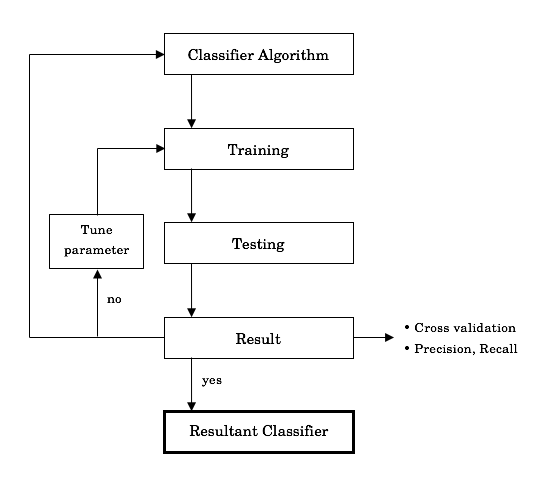
\includegraphics[scale=0.6]{supervised-process.png}
  \caption{An overview of the process for getting a supervised classifier~\cite{class-analysis}}
  \label{fig:supervised-process}
\end{figure}

Supervised learning is ideal when there are an abundance of correctly labelled data for the classifier to learn from. Figure~\ref{fig:supervised-process} describes this graphically. A \textit{training set} contains some pre-labelled data which the classifier algorithm will be trained on. Some of the pre-labelled data is set aside and used as the \textit{test set} to see how well the trained classifier performs. 


\subsection{Unsupervised Classification}
Unsupervised classification is also known as clustering. Items with similar properties in the data level will be grouped together by the algorithm itself. Training is still required, otherwise the classifier will not be able to put a label to an unknown item. The training data should be unlabelled, to allow the algorithm decide on the number of clusters (labels). Ultimately, the goal with unsupervised learning is to avoid any intervention and let the algorithm does its job \cite{hall-notes}. 

This should not be confused with \textit{online learning}. An unsupervised classifier does not 

\subsection{NYU Depth Dataset V2}
Quality training data is required to achieve high precision and accuracy. The NYU Depth Dataset provides a quality wide range set of depth data which can be used for training a classifier with the aim of achieving high precision and accuracy. There are 1449 densely labelled and 407 024 unlabelled newly scenes in this version. The large amount of wide variety of scenes and items of the same class is ideal to be used as training data \cite{nyu-dataset}.

The abundance of available data means that time can be saved from having to locate many objects of the same in different scene settings, but effort can be focussed in getting the \textit{best} 

% Integrating Kinect Depth Data with a Stochastic Object Classification Framework for Forestry Robot

\section{Machine-learning in Python}
\subsection{\texttt{scikit-learn}}
\texttt{scikit-learn} is a machine-learning library for Python, which is actively in development. It has quality implementations of popular machine-learning algorithms for different machine-learning problems. It is built on \texttt{numpy} and \texttt{scipy}, making it easy for data manipulation \cite{scikit-learn-paper}. A wide range of companies and researches use scikit learn for machine-learning purposes, including Spotify and Evernote.\footnote{\url{http://scikit-learn.org/stable/testimonials/testimonials.html}} Pedregosa et al. \cite{scikit-learn-paper} copmared it with other Python machine-learning packages which sees scikit-learn beating the others in baseline tests.

Supported supervised classification algorithms include Support Vector Machines (SVM), Random Forest, Stochastic Gradient Descent, Nearest Neighbours and Decision Tree. 

\subsubsection{R, MatLab}
\textit{incomplete...}

\section{Performance}
\subsection{Precision and Recall}
The precision and recall rates (accuracy) can be calculated to analyse the performance of the classifier.~\cite{precision-recall} They are calculated by comparing predictions against the actual values.

\parbox{\linewidth} {
  \centering
  \begin{tabular}{|l|c|c|}
    \hline
                        & Actual Positive & Actual Negative
    \\ \hline
    Predicted Positive  & TP              & FP
    \\ \hline
    Predicted Negative  & FN              & TN
    \\ \hline
  \end{tabular}

  \captionof{table}{Confusion matrix (taken from~\cite{precision-recall})}
  \label{tab:cm}
}

In order to calculate these rates, a confusion matrix is computed. It is a table that puts the correctness of predictions against the actual values of the underlying data (Table~\ref{tab:cm}). This shows the number of correct and incorrect recognition, allowing a couple of metrics to be calculated, notably precision and recall. (Table~\ref{tab:eq}) 

\parbox{\linewidth} {
  \centering
  \begin{tabular}{|l|}
    \hline \\
    \( Recall              = \frac{TP}{TP + FN} \) \\[10pt]
    \( Precision           = \frac{TP}{TP + FP} \) \\[10pt]
    \( True Positive Rate  = \frac{TP}{TP + FN} \) \\[10pt]
    \( False Positive Rate = \frac{FP}{FP + TN} \) \\~\\
    \hline
  \end{tabular}
  
  \captionof{table}{Common machine-learning evaluation metrics (taken from~\cite{precision-recall})}
  \label{tab:eq}
}

Precision can be described as \textit{"out of the predicted positives/ negatives, how much did the prediction is correct" }, whereas recall is described as \textit{"out of the actual positives/ negatives, how much did the prediction is correct"}, as seen in Table~\ref{tab:eq}. The former tells us how well the model can predict correctly; the latter tells us the \textit{quantity} of which the relevant items is picked.~\cite{precision-recall-wiki}

To say that a model is \textit{good for use}, it has to be both precise and has a high recall rate. If a model is very precise, but does not pick up much of the relevant items, the model might look as if it was performing well, but in fact, it hardly picked up enough of the right items; vice versa.

\subsection{Cross-validation}
It is important to ensure that the training and testing sets are different and that there is no overlap between the two sets, otherwise overfitting will happen. Overfitting is evident when a classifier appears to be functioning perfectly during the train-and-test stage, but turns out to be unable to classify new objects when put into use. On top of the training and test sets, a third validation subset can be introduced. This enables an extra check to ensure that the classifier actually works.  However, the precision and accuracy of the classifer could suffer as a result of a smaller training set \cite{cross-val-scikit}. 

Cross-validation solves the problem by creating some \textit{mutually exclusive} folds (subsets). These folds are created after a test set is taken out from the original set of data. One popular algorithm is \textit{k}-fold cross-validation. It does not run validation on all possible splits on the folds but one different split for each run to save on computational complexity. Multiple cross-validation runs with different splits are performed, resulting in an average that estimates the complete cross-validation \cite{cross-val-kohavi}. This gives an unbiased view as to how the classifier performs, as it is not limited to one fixed set of testing data.

\subsection{Statistical Testings}
TG Dietterich \cite{t-test-paper} proposed five statistical t-tests that can be used to compare different supervised classification algorithms. Statistical testings provide a good way to unbiasedly compare different algorithms and see how they actually perform in a particular situation.

\textit{TODO: read the paper in detail and find other relevant sources about other statistical tests that could be used\cite{t-test-paper}}


\newpage
\section{Classification Algorithms}
In this section, we focus on what scikit-learn can offer with its implementations of some of the most popular algorithms.

\subsection{Notable Supervised Algorithms}

\texttt{scikit-learn} supports many supervised algorithms and 
\begin{itemize}
  \item \textbf{Stochastic Gradient Descent (SGD)} fits a linear model efficiently and is particularly useful when there is a wide and large dataset for training. 
  \item \textbf{Support Vector Machines (SVM)} enabels multi-class classification with different algorithms based on the nature of the kernel. Some examples are linear SVM and RBF SVM (1.4 \cite{scikit-docs-supervised}.
  \item \textbf{Nearest Neighbours (NN)} has a number of implementation with \texttt{scikit-learn}. In general, works well with larger datasets. It could reduce noise but blur the boundaries of the clusters, making it harder to distinguish between labels (1.6.2 \cite{scikit-doccs-supervised}). 
  \item \texttt{scikit-learn} uses an implementation of the CART \textbf{Decision Tree (DT)}. It extends C4.5, a well-regarded implementation with high accuracy while adding support to regression and other features (1.10.6 \cite{scikit-docs-supervised}). 
  \item \textbf{Random Forest (RF)} has many trees. They are built by the best split within a random subset. The result is based on the average of these predictions (1.11.2 \cite{scikit-docs-supervised}).
\end{itemize}

\parbox{\linewidth}{
  \centering
  \begin{tabular}{|c|c|c|c|c|}
    \hline
    Model    & Calibration & Training Speed  & Fast at Classifying & Mean Accuracy
    \\\hline
    BST-DT   & PLT         & Slower than DT  & ?                   & 0.917
    \\\hline
    RF       & PLT         & Faster than SVM & ?                   & 0.898
    \\\hline
    SVM      & -           & Slow            & ?                   & 0.880
    \\\hline
    DT       & ISO         & YES             & ?                   & 0.774
    \\\hline
  \end{tabular}

  \captionof{table}{Comparing properties of different classification models (accuracy information from \cite{compare-supervised}}
  \label{tab:comparison}
}

Table~\ref{tab:comparison} shows some of the empirical comparison results done by Caruana and Niculescu-Mizil \cite{compare-supervised}. 11 binary tests are performed and their averages of the outcome form the accuracy rates for each of the classifiers. As different algorithms have different characteristics and are fit for different purposes, calibration with algorithms such as isotonic regression aims to provide an unbiased view on how well the algorithms perform.

It shows that boosted tree performed the best while Random Forest performed better than SVM. There is some discrepancy between this and \texttt{scikit-learn}'s documentation \cite{scikit-docs-supervised-compare}. The documentation shows that the SVM implementations in \texttt{scikit-learn} has the best performance. 

SVM is known to not scale well and train slowly. If the results provided in \cite{compare-supervised} is trust-worthy, there is little incentive to use a slow algorithm that does not boost precision and accuracy. It is also known that a Linear SVM, which is used by \cite{compare-supervised} does not perform well if the clusters are closely packed together. This could explain the discrepancy.

\subsection{Notable Unsupervised Algorithms}
\textit{TODO: describe and compare k-means, mean-shift, DBSCAN}


\section{Using Classifiers for Depth Data}
\textit{TODO: Discuss how Naive Bayes, Decision Trees and SVMs are used in the Forestry Robot paper \cite{forestry}}

\textit{TODO: segmentation using online learning with a real-time random forest algorithm in Semantic Paint \cite{semantic-paint}}

\newpage

% summary
\chapter{The Project}
When creating the classifier, it is important to conduct many tests to ensure it is performing properly and well. As discussed, precision and recall, cross-validation and statistical testing are helpful tools to help achieve a good should also be done to ensure that the classifier performs properly based on an unbiased view. 

It is reckoned that the performance at classifying a scene is more important than the time required at training. The trade-off between training time and precision and recall is little, so it is worth trying Gradient Boosting Classier (Boosted Tree), Random Forest and SVM to try to obtain the highest accuracy and low false positive/negative rates. Simple Decision Trees seem to perform less well compared to the others. 

\textit{TODO: discuss if using multiple classifiers and combining the results like \cite{forestry} should be approached}

\textit{TODO: discuss how to use segmentation methods described by Semantic Paint \cite{semantic-paint} and the NYU Dataset research \cite{nyu-dataset}}.

\newpage


% bibliography
\pagenumbering{gobble}
\bibliographystyle{unsrt}
\bibliography{mybib}


\end{document}
